% ----------------------------------------------------------
% Introdução (exemplo de capítulo sem numeração, mas presente no Sumário)
% ----------------------------------------------------------
\chapter{Introdução}
\label{cap-introducao}
% ----------------------------------------------------------
Muito tem se discutido sobre os impactos negativos causados pelo homem ao meio-ambiente, motivados em grande parte pelo exagerado consumo dos recursos naturais. Também é crescente a busca por novas formas de obtenção destes recursos de forma a evitar a escassez ou o fim dos mesmos. Ora, esta escassez é principalmente causada pelo avanço das industrias e aumento da população global. Dentro deste contexto a energia elétrica é um subsídio crucial pois é essencial tanto para o processo produtivo quanto para manutenção da existência humana.

Segundo \citeonline[p.~300]{Bassanezi2002} a modelagem é muito importante.

Consciente desta escassez o homem desenvolveu diferentes formas de obter energia. Segundo \citeonline[p.~9]{Goldemberg2007} as fontes de energia são classificadas como renováveis e não-renováveis (ou seja, recursos finitos). Dentre as diversas fontes de energias renováveis, a energia solar destaca-se por ser a mais abundante, limpa e de fácil obtenção. Através da instalação de painéis fotovoltaicos (tecnologia que permite a conversão da radiação solar em energia elétrica) pessoas e empresas têm buscado redução dos custos energéticos e também uma maneira de poupar os recursos não-renováveis.


Segundo \citeonline[p.~300]{Bassanezi2002} a modelagem é muito importante.

Este projeto visou o desenvolvimento de um sistema para apoio ao dimensionamento dos sistemas de energia solar, além de possibilitar o armazenamento e controle de informações da comercialização (clientes, materiais, etc.). A escolha do tema levou em consideração o atual momento aonde tem aumentado o interesse por fontes renováveis de energia ao mesmo tempo em que tem diminuído os custos relativos a implantação dos sistemas fotovoltaicos.


Segundo \citeonline[p.~300]{Bassanezi2002} a modelagem é muito importante.

Como estratégia optou-se pelo desenvolvimento de uma aplicação web utilizando a linguagem Java e diversas outras tecnologias, incluindo o banco de dados open-source PostgreSQL. A implantação da aplicação foi realizada principalmente no serviço de computação em nuvem da Amazon Web Services (AWS), utilizando alguns dos diversos recursos oferecidos pela plataforma. A aplicação foi desenvolvida de forma distribuída, sendo composta por uma aplicação web principal e dois serviços web API REST. 


Segundo \citeonline[p.~300]{Bassanezi2002} a modelagem é muito importante.

\section{Objetivo Geral}

O objetivo deste trabalho é desenvolver uma aplicação para o dimensionamento de sistemas de energia fotovoltaica, utilizando tecnologia web em uma arquitetura de sistema distribuído.

\section{Objetivos Específicos}

O trabalho terá os seguintes objetivos específicos:

Relativo ao negócio:
\begin{itemize}
	\item Controlar o cadastro de clientes e materiais de energia fotovoltaica.
	\item Realizar o dimensionamento do sistema solar para efetuar orçamento, baseando-se nas necessidades do cliente versus os materiais cadastrados disponíveis.
	\item Enviar link do orçamento via e-mail, permitindo assim que o cliente visualize ou imprima o documento, conforme desejar.
\end{itemize}

Relativo à tecnologia:
\begin{itemize}
	\item Selecionar as tecnologias que irão compor o software estabelecendo assim a arquitetura do sistema.
	\item Desenvolver um software distribuído com base na arquitetura estabelecida.
	\item Manter algumas configurações da aplicação (parâmetros simples do sistema, tais como: urls, constantes, etc.) ajustáveis através de interface, para futuros alterações sem necessidade de recompilar.
	\item Proteger aplicação através de controle de acesso.
\end{itemize}

\section{Justificativa}

%TODO
Atualmente a quantidade de instalações de sistemas de energia fotovoltaica têm crescido de forma significativa, \citeonline[online]{estadao_2018} afirma que houve um crescimento de 407\% entre os anos de 2017 e 2018 neste setor, e que para os próximos anos, a tendência é que este crescimento continue. Ainda, de acordo com \citeonline[p.~82]{aneel_2008} a utilização mundial de energia solar cresceu 2.000\% entre 1996 e 2006.

\begin{citacao}
	O Brasil possui expressivo potencial para geração de energia elétrica a partir de fonte solar, contando com níveis de irradiação solar superiores aos de países onde projetos para aproveitamento de energia solar são amplamente disseminados, como Alemanha, França e Espanha \cite[p.~4]{nascimento2017energia}.
\end{citacao}

Através da \autoref{fig_aumento-utilizacao-energia-solar-2014} observa-se o significativo aumento do uso da energia solar em diferentes setores como residencial, comercial e larga escala.

\begin{figure}[htb]
	\caption{\label{fig_aumento-utilizacao-energia-solar-2014}Aumento da utilização da energia solar em diferentes setores}
	\begin{center}
		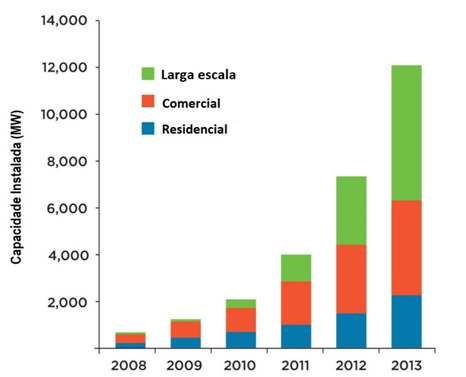
\includegraphics[scale=0.8]{introducao/imagens/aumento-utilizacao-energia-solar-2014.PNG}
	\end{center}
	\legend{Fonte: Adaptado de \citeonline[p. 9]{rogers2014solar}}
\end{figure}

Outro dado importante é a constante redução do custo com a implantação dos sistemas, a maior parte deste custo geralmente é destinada a obtenção dos equipamentos necessários. De acordo com \apudonline[p.~33]{epe2016compromisso}{nascimento2017energia} os custos de instalação de painéis fotovoltaicos se reduzirão cerca de 30\% até 2020 e 50\% até 2030. Esta redução dos custos tem contribuído para a popularização e o aumento da quantidade de instalações de sistemas de energia fotovoltaica. Na \autoref{fig_reducao-preco-painel-solar-2014} é possível visualizar a significativa redução no preço dos painéis fotovoltaicos ao longo dos anos.

\begin{figure}[htb]
	\caption{\label{fig_reducao-preco-painel-solar-2014}Redução do preço dos painéis solares em diferentes setores}
	\begin{center}
		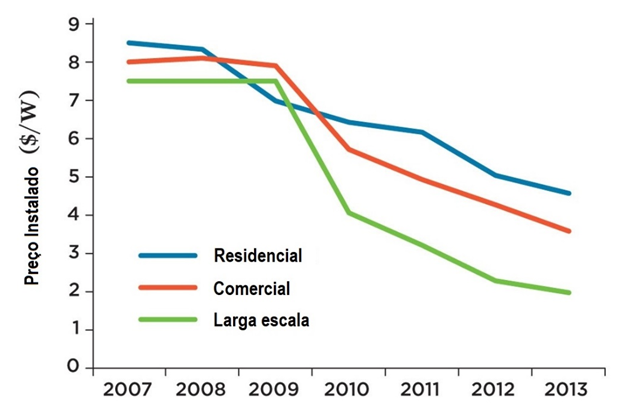
\includegraphics[scale=0.6]{introducao/imagens/reducao-preco-painel-solar-2014.PNG}
	\end{center}
	\legend{Fonte: Adaptado de \citeonline[p. 5]{rogers2014solar}}
\end{figure}

Diante destes fatos, considera-se plausível o desenvolvimento deste projeto, uma vez que o cenário se encontra favorável às tecnologias ligadas a energia solar.

\section{Organização do Trabalho}

Este trabalho é composto por cinco Capítulos, organizados da seguinte forma: após uma introdução no \autoref{cap-introducao}, o \autoref{cap_revisao_bibliografica} apresenta os conceitos e definições necessários para entendimento desta pesquisa. No Capítulo 3 será abordada a metodologia utilizada no trabalho. O Capítulo 4 por sua vez mostrará como foi o desenvolvimento de todo o trabalho com base na Metodologia e ressaltando todos os passos do processo. Por fim, no Capítulo 5 serão apresentados os possíveis trabalhos futuros e a conclusão deste trabalho.


% Exemplo de citação e referencia de quadros

% \begin{quadro}[htb]
% \caption{\label{quadro_exemplo}Exemplo de quadro}
% \begin{tabular}{c|c|c|c}
% 	%\hline
% 	\textbf{Pessoa} & \textbf{Idade} & \textbf{Peso} & \textbf{Altura} \\ \hline
% 	Marcos & 26    & 68   & 178    \\ \hline
% 	Ivone  & 22    & 57   & 162    \\ \hline
% 	...    & ...   & ...  & ...    \\ \hline
% 	Sueli  & 40    & 65   & 153   % \\ \hline
% \end{tabular}
% \fonte{Autor.}
% \end{quadro}

% Primeira opção, utilizando \texttt{autoref}: Ver o \autoref{quadro_exemplo}. 
% Segunda opção, utilizando  \texttt{ref}: Ver o Quadro \ref{quadro_exemplo}.

%--------
